\documentclass{article}
\usepackage[letterpaper,portrait,top=0.4in, left=0.6in, right=0.6in, bottom=1in]{geometry}

\usepackage{amsmath, amsfonts, amsthm, amssymb}
\usepackage{graphicx, float}
\usepackage{suffix}
\usepackage{esdiff}
\usepackage{multicol}
\usepackage{cancel}
\usepackage{mdframed}
\usepackage{mathtools}
\usepackage{tcolorbox}
\usepackage{hyperref}
\usepackage[per-mode=symbol]{siunitx}
\usepackage{setspace}
\usepackage{parskip}
\usepackage{titling}
\usepackage{mlmodern}

\newcommand{\alignedintertext}[1]{%
  \noalign{%
    \vtop{\hsize=\linewidth#1\par
    \expandafter}%
    \expandafter\prevdepth\the\prevdepth
  }%
}

\newcommand{\definition}[1]{\begin{tcolorbox}[colback=red!5!white,colframe=red!75!black,parbox=false] #1 \end{tcolorbox}}

\newcommand{\theorem}[2]{\begin{tcolorbox}[title={#1},colback=blue!5!white,colframe=blue!75!black,parbox=false] #2 \end{tcolorbox}}
\WithSuffix\newcommand\theorem*[1]{\begin{tcolorbox}[colback=blue!5!white,colframe=blue!75!black,parbox=false] #1 \end{tcolorbox}}

\newcommand{\example}[2]{\begin{tcolorbox}[title={Example: #1},colback=brown!5!white,colframe=brown!75!black,parbox=false] #2 \end{tcolorbox}}

\newcommand{\remark}[2]{\begin{tcolorbox}[title={#1},colback=black!5!white,colframe=black!75!black,parbox=false] #2 \end{tcolorbox}}
\WithSuffix\newcommand\remark*[1]{\begin{tcolorbox}[colback=black!5!white,colframe=black!75!black,parbox=false] #1 \end{tcolorbox}}

\newcommand*{\deriv}[1][x]{\ensuremath{\dfrac{\mathrm{d}}{\mathrm{d}#1}}}
\newcommand*{\floor}[1]{\ensuremath{\lfloor #1\rfloor}}

\title{\vspace*{-40pt}AP Physics C -- Class Notes}
\author{Jayden Li}
\date{\today}

\begin{document}
\setstretch{1.25}
\fontsize{11pt}{12pt}\selectfont
\setlength{\abovedisplayskip}{\abovedisplayskip/2}
\setlength{\belowdisplayskip}{\belowdisplayskip/2}
\setlength{\parindent}{0pt}
\setlength{\parskip}{2ex plus 0.5ex minus 0.2ex}
\maketitle

\tableofcontents
% \newpage

\section{Introduction}

\subsection{Jumping Monsters}

See Figure 1.1 in Notebook.

We investigate the relationship between the mass of the toy $m$ and the change in height $\Delta h$. Equipment:
\begin{itemize}
	\item Meter stick (not ruler, since ruler is only 30cm long)
	\item Phone (to record video)
	\item Balance (to measure mass in grams and kilograms, a scale measures weight in Newtons)
	\item Washers, paper clips and tape (to increase mass of toy)
\end{itemize}

We collect many data points. We will collect 5 data points, which is 5 conditions, which is 5 different masses to test.  We want to repeat every mass a few times too; we will test every mass 3 times (``3 trials''). In total, the toy will jump $5\cdot 3=15$ times. Trial means that conditions/masses are the same.

Results/data are in Table 1.2 in Notebook.

Based on conservation of energy:
\begin{equation*}
    \text{PE}_ \text{s}= \text{PE}_ \text{g}
	\implies \frac12kx^2=mgh
	\implies h=\frac{kx^2}{2mg}=\frac{kx^2}{2g}\cdot\frac1m
\end{equation*}
If we graph mass $m$ against height $\Delta h$, this is an inverse relationship, as $kx^2/2g$ is a constant (the spring distance $x$ does not change for one toy, $k$ is spring constant, and $g$ is acceleration due to gravity).

Because we want a linear relationship, we can graph inverse mass $1/m$ against height $\Delta h$. This becomes a line with slope $kx^2/2g$.

Logger pro graph, plotting inverse mass in $1/\text{kg}$ against height in meters:

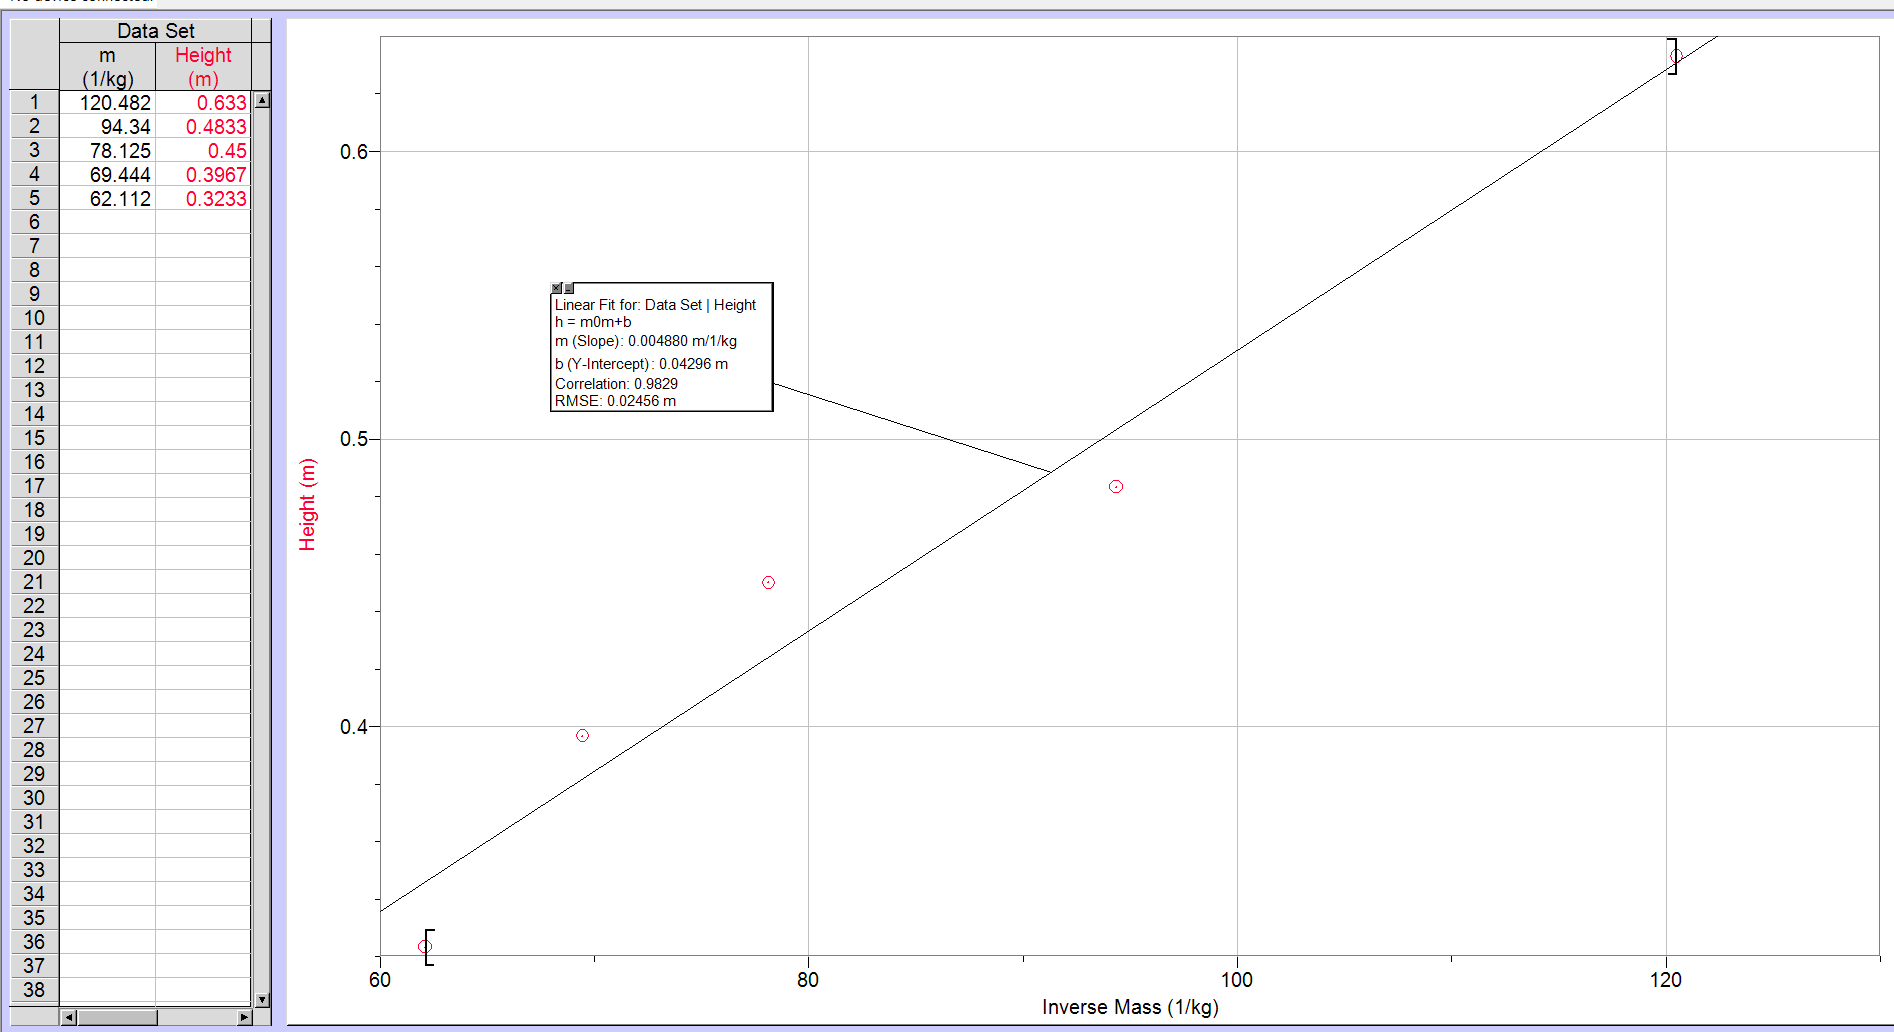
\includegraphics[width=\linewidth]{loggerpro0903.png}
\begin{equation*}
	\text{Slope}
	=m 
	=\frac{kx^2}{2g}
	=0.004880
	\implies k=m\cdot \frac{2g}{x^2}
	=0.004880\cdot \frac{2(9.81)}{(1.5/100)^2}
	=\boxed{425.536\,\si{\newton\per\meter}}
\end{equation*}

\remark{Linearization}{Linearization is a powerful technique. For example, with Kepler's third law of planetary motion:
\begin{equation*}
    \frac{T^2}{r^3}=\frac{4\pi^2}{GM}
\end{equation*}
is annoying to plot when we plot $T$ against $r$. We rearrange and plot $T^2$ against $r^3$ for a linear relationship:
\begin{equation*}
    T^2=\frac{4\pi^2}{GM}r^3
\end{equation*}
$4\pi^2/GM$ is a constant/the slope. We take $y=T^2$ and $x=r^3$, and we have the fitted slope $m=4\pi^2/GM$.}

\subsection{Projectile Motion}

Two-dimensional motion, $x$ and $y$-directions. The type of motion in the two directions are different.

$x$-direction has constant velocity because there is no net force and no acceleration acting in the $x$-direction.
\begin{equation*}
    v_x=\frac{\Delta x}{\Delta t}
	\iff \Delta x=v_x(\Delta t)
\end{equation*}

$y$-direction has constant acceleration due to gravity $-g$.
\begin{align*}
	v_y&=v_{0y}+at \\
	\Delta y&=v_{0y}t+\frac12at^2 \\
	v_y^2&=v+{0y}^2+2a\Delta y
\end{align*}

\subsubsection{Special cases}

In horizontal projectile motion, $v_{0y}=0\,\si{\meter\per\second}$.

When the projectile reaches its highest point in general 2-dimensional motion, then at the highest point, there is no $y$-velocity: $v_y=0\,\si{\meter\per\second}$.

If the projectile is launched at a certain velocity $v_0$ at an angle $\theta$, we have initial $x$ and initial $y$-velocities:
\begin{align*}
	v_x=v_{0x}&=v_0\cos\theta \\
	v_{0y}&=v_0\sin\theta
\end{align*}

\subsection{Momentum Lab}

Equipment:
\begin{itemize}
	\item Motion sensor/detector
	\item Force sensor: measures force
	\item Cart connected to plunger; plunger is a metal rod with a spring inside
\end{itemize}

Push cart on a track, measure force and velocity to obtain the mass of the cart. To improve the accuracy and lower the percent error:
\begin{itemize}
	\item Check if the track is level, if the track is inclined then the cart is not moving at a constant velocity (disregarding friction) before and after the collision.
	\item Reduce friction
	\item Increase the number of \textbf{experimental conditions} (cannot increase the number of trials, because trial has the same conditions like initial speed, which is not possible to make sure) by pushing it more times
	\item Line up force sensor and cart/track
\end{itemize}

\subsection{AP Formula Sheet}

$G$ universal gravitational constant is important. We should take acceleration due to gravity on Earth $g=10\,\si{\meter\per\second\squared}$. Magnitude of gravitational field of earth is also $g=10\,\si{\newton\per\kilo\gram}$. These units are equivalent.

Kinematic equations for \textbf{constant acceleration} and therefore constant force:
\begin{equation*}
    \Delta x=v_0t+\frac12at^2 \qquad
	v=v_0+at \qquad
	v^2=v_0^2+2a\Delta x
\end{equation*}
Newton's second law does not have to be complicated; $\Sigma F=ma$ is fine.

Maximum friction $\lVert \vec{F}_f \rVert =\lVert \mu \vec{F}_N \rVert $ tells us, where $\vec{F}_N$ is normal force:
\begin{itemize}
	\item kinetic friction $\vec{F}_k=\mu_k \vec{F}_N$
	\item Maximum static friction $\vec{F}_\text{s,max}=\mu_\text{s,max}\vec{F}_N$
	\item Static friction $\lVert \vec{F}_\text{s} \rVert <\vec{F}_\text{s,max}$.
\end{itemize}

\section{Calculus}

\subsection{Calculus-Based Equations}

\theorem{Kinematics}{
	\begin{alignat*}{2}
		v&=\diff xt &\qquad \Delta x=\int v\,\mathrm{d}t \\
		a&=\diff vt=\diff[2]{x}{t} &\qquad \Delta v=\int a\,\mathrm{d}t
	\end{alignat*}
	where $x$ is position, $v$ is velocity and $a$ is acceleration. These will apply to all situations (for constant velocity, constant acceleration or nonconstant acceleration).
}

Integrate with respect to independent variable; integrand is dependent variable. See Figure 2.1.

\theorem{Connecting dynamics/forces and kinematics}{
Newton's second law: $\Sigma F=ma$. Acceleration $a$ connects forces and dynamics to kinematics.

Suppose we are given position $x$. Then we can calculate the acceleration by differentiation:
\begin{equation*}
	a=\diff[2]xt
	\implies F=ma=m\diff[2]xt
\end{equation*}
}

Connecting energy and kinematics by kinetic energy $K=mv^2/2$.

\theorem{Work and force-position graphs}{
	Consider a force-position graph (Figure 2.2). The area under the curve is the work done, or change in energy: $W=\Delta E$. The relationship is as follows, where $\Sigma F$ is the net force:
	\begin{equation*}
	    \Delta E=\int\Sigma  F\,\mathrm{d}x
		\qquad \Sigma F=\diff Ex
	\end{equation*}
}

\theorem{Power and time}{
	Power is the rate of change of energy with respect to time:
	\begin{equation*}
		\Delta E=\int P\,\mathrm{d}t \qquad P=\diff Et
	\end{equation*}
	The change in energy is the area under the curve of a power-time graph (Figure 3.3).
}

\theorem{Force and time}{
	Recall that for constant net force $\Sigma F$, impulse $J=\Delta p=\Sigma F\cdot \Delta t$. For a force-time graph in Figure 2.4:
	\begin{equation*}
	    J=\Delta p=\int F\,\mathrm{d}t
		\qquad 
		F=\diff{p}{t}=m\cdot \diff vt=ma
	\end{equation*}
	(Impulse $\Delta p=I=J=\Delta(mv)=m \cdot \Delta v$, since mass usually does not change. $\mathrm{d}p=F\mathrm{d} t \implies \mathrm{d}(mv)=m\mathrm{d} v=F\mathrm{d} t\implies F=m(\mathrm{d}v/\mathrm{d}t)=ma$)
}

\theorem{Rotational kinematics}{
	\begin{equation*}
		\omega=\diff{\theta}t \qquad
		\alpha=\diff{\omega}{t} \qquad
		\Delta\theta=\int \omega\,\mathrm{d}t \qquad
		\Delta \omega=\int \alpha\,\mathrm{d}t
	\end{equation*}
}

\subsection{Potential Energy}

Suppose we drop a ball from a certain height. We know that the work done by the force of gravity is positive work, but since energy is conserved, the potential energy in the ball must decrease. Therefore, we have:
\begin{equation*}
    -W=\Delta U 
\end{equation*}
But, we know that work is force times distance:
\begin{equation*}
	\Delta U=-F_y\cdot \Delta y
	\implies F_y=-\frac{\Delta U}{\Delta y}
\end{equation*}
where $\Delta y$ is the distance the ball is dropped, or the distance over which the force acts. By black magic, we can change this into a derivative:
\begin{equation*}
	F_y=-\diff Uy
\end{equation*}
Must have negative sign. So, we can also have potential energy in terms of force:
\begin{equation*}
    F_y=-\diff Uy
	\implies -F_y \,\mathrm{d}y=\mathrm{d}U
	\implies \Delta U=-\int F_y\,\mathrm{d}y
\end{equation*}
\remark*{In nature, objects want to lower their potential energy. (NOTE: lower the number, NOT the magnitude of kinetic energy.)}

\theorem{Potential energy}{
	The relationship between potential energy and force is, where $x$ is position:
	\begin{equation*}
	    \Delta U_x=-\int F_x\,\mathrm{d}x
		\qquad
		F_x=-\diff Ux
	\end{equation*}
}

In simple harmonic motion, the potential energy-displacement from equilibrium graph is a positive parabola passing through the origin. There is no potential energy at equilibrium ($x=0$) and potential energy is maximized at the highest displacement.

Total energy is the sum of kinetic energy and potential energy: $K+U$. By conservation of energy, the total energy is constant for all displacement.

\definition{The work done by a \textbf{conservative force} only depends on the initial and final position of the object, not on the path taken.}

A lot of forces are path-dependent. For example, friction depends on the length of the path, so it is not conservative. Forces associated with change in potential energy are conservative.

\example{Gravitional potential}{
	Change in gravitational potential energy is $\Delta U_g=mgy$. We can calculate the force:
	\begin{equation*}
		F_g=-\diff{U_g}{y}=-\deriv[y](mgy)=-mg
	\end{equation*}
	is consistent with the result we get from $F=ma$.
}

\example{Spring potential}{
	Change in spring potential is $U_s=kx^2/2$:
	\begin{equation*}
		F_s=-\diff{U_s}{x}=-\deriv[x]\left(\frac12kx^2\right)=-kx
	\end{equation*}
}

\subsection{Springs}

Formulas like $F_s=-kx$ and $U_s=kx^2/2$ depend on a \textbf{perfect, ideal spring}, which requires some assumptions.
\begin{itemize}
	\item The mass of the spring itself is negligible; the mass of the system is exactly the mass of the object attachde to the spring.
	\item Force exerted is $F_s=-kx$: force-displacement graph is linear and passes through the origin. From this, formula for kinetic energy follows: $U_s=-\int F_s\,\mathrm{d}x=-\int -kx\,\mathrm{d}x=kx^2/2$.
	\item No internal friction and losses. If there are, \textit{damping} occurs. This is drawn in Figure 2.5. Even though the period does not change, each successive crest and trough decreases in magnitude.
\end{itemize}

Figure 2.6 shows the energy position graph of an ideal spring. By conservation of energy, total energy $\text{TE}=U_s+K$.

Real springs are non-ideal.

\section{Conservation of Momentum}

\subsection{Explosions}

\definition{An explosion is when two objects separate after being together.}

Cart of mass $m_1$ and mass $m_2$ separate after a compressed spring between them, and they move at velocity $v_1$ and $v_2$. $m_1>m_2$. By conservation of momentum:
\begin{equation*}
    m_1v_1=m_2v_2
	\implies v_2=\frac{m_1v_1}{m_2}
\end{equation*}
We calculate each object's kinetic energy:
\begin{align*}
	K_1&=\frac12m_1v_1^2 \\
	K_2&=\frac12m_2v_2^2
	   =\frac12m_2 \left( \frac{m_1v_1}{m_2} \right)^2
	   =\frac12 m_1\left(\frac{m_1}{m_2}\right)v_1^2
	   =\frac{m_1}{m_2}K_1
\end{align*}
Since $m_1>m_2$: $m_1/m_2>1\implies K_2>K_1$

\theorem*{If momentum is conserved after a collision or explosion, then the object with the lower mass (and therefore higher velocity) has higher kinetic energy.}

\subsection{Elastic Head-On Collisions}

\definition{In a head-on collisions, both objects are moving in a straight line. In a glancing collision, objects will go in different angles after the collision.}

Suppose that two objects collide head on. The objects are initially traveling at velocities $v_1,v_2$, and have velocities $v_1',v_2'$ after the collision.

By conservation of momentum and conservation of kinetic energy (because collision is elastic):
\begin{align*}
	\Sigma p&=\Sigma p' \\
	m_1v_1+m_2v_2&=m_1(v_1')+m_2(v_2') \tag{1} \\
	\frac12m_1v_1^2+\frac12m_2v_2^2&=\frac12m_1(v_1')^2+\frac12m_2(v_2')^2 \tag{2}
\end{align*}
We can use this to derive another equation:
\begin{align*}
	(2)
	&\implies \frac12m_1v_1^2+\frac12m_2v_2^2=\frac12m_1(v_1')^2+\frac12m_2(v_2')^2
	\implies m_1v_1^2+m_2v_2^2=m_1(v_1')^2+m_2(v_2')^2 \\
	&\implies m_1 v_1^2-m_1(v_1')^2=m_2(v_2')^2-m_2v_2^2
	\implies m_1 \left( v_1^2-(v_1')^2 \right)=m_2 \left( (v_2')^2-v_2^2 \right) \\
	&\implies m_1(v_1+v_1')(v_1-v_1')=m_2(v_2'+v_2)(v_2'-v_2) \\
	(1)
	&\implies m_1v_1-m_1(v_1')=m_2(v_2')-m_2v_2
	\implies m_1 \left( v_1-v_1' \right)=m_2 \left( v_2'-v_2 \right) \\
	\frac{(2)}{(1)}
	&\implies \frac{\bcancel{m_1}(v_1+v_1')(\cancel{v_1-v_1'})}{\bcancel{m_1}(\cancel{v_1-v_1'})}=\frac{\bcancel{m_2}(v_2'+v_2)(\cancel{v_2'-v_2})}{\bcancel{m_2}(\cancel{v_2'-v_2})}
	\implies v_1+v_1'=v_2+v_2'
\end{align*}

\theorem{Equations for a head-on elastic collision}{
	\begin{align*}
		m_1v_1+m_2v_2&=m_1(v_1')+m_2(v_2') \tag{Conservation of Momentum} \\
		\frac12m_1v_1^2+\frac12m_2v_2^2&=\frac12m_1(v_1')^2+\frac12m_2(v_2')^2 \tag{Conservation of Kinetic Energy} \\
		v_1+v_1'&=v_2+v_2'
	\end{align*}
}

\subsection{Ballistic Pendulum}

Bullet of mass $m$ into a block of mass $M$ at velocity $v$. The bullet lodges into the mass and travels with the block. This is a completely inelastic collision.

We can calculate the final velocity of the block by conservation of momentum $mv=(M+m)V$. From $V$ we can calculate the kinetic energy $K$, and gravitational potential energy when the block is shot is $0$. So the total mechanical energy is $K+0=K$.

The highest point in the pendulum is reached when the gravitational potential energy equals the total energy:
\begin{equation*}
	\frac12(\cancel{M+m})V^2=(\cancel{M+m})g\Delta h
	\implies \Delta h=\frac{V^2}{2g}
\end{equation*}

\subsection*{Free Response Questions}

\remark{Free response}{\begin{itemize}
	\item Use pencil or black/blue pen.
	\item Start by writing known equation.
	\item Substitution (substitute numbers with no units).
	\item Final answer clearly indicated such as \boxed{\text{boxed}}.
		\begin{itemize}
			\item If numerical, do not keep infinite number of significant figures: no square root, fraction, constants; \textbf{always 2 or 3 significant figures, never 1 s.f.!!!!!}
			\item If symbolic, leave square roots, fractions, constants:
		\end{itemize}
	\item Graphing: label axes with units:
		\begin{itemize}
			\item Name of graph is ``[value on $y$ axis] vs [value on $x$ axis]'' or ``[value on $y$] wrt [value on $x$]''.
			\item Line of best fit: equal number of points above and below the line.
			\item When determining slope of line of best fit, do not choose original values: $\text{Slope}=\Delta y/\Delta x=(y_1-y_0)/(x_1-x_0)$. \textbf{The slope has units.}
		\end{itemize}
	\item Integrals: must have limits of integration and differential.
\end{itemize}}

\subsection{Center of Mass}

\end{document}

